\documentclass[12pt,a4paper]{report}
\usepackage[utf8]{inputenc}
\usepackage[spanish]{babel}
\usepackage{amsmath}
\usepackage{tikz}
\usepackage{amsfonts}
\usepackage{amssymb}
\usepackage{graphicx}
\usepackage[left=2cm,right=2cm,top=2cm,bottom=2cm]{geometry}
\author{Marcos Rivera Almazo}
\title{ as}
\begin{document}

\begin{center}
{\huge Solución numérica del átomo de Hidrógeno usando el método de Numerov}\\
\vspace{0.5cm}
{\Large Marcos Rivera Almazo}
\end{center}

\subsection*{Introducción}

La ecuación de Schrödinger para el átomo de Hidrógeno, en unidades atómicas y coordenadas esféricas, tiene la siguiente forma:

\begin{equation}\label{hsh}
-\frac{1}{2}\nabla^2 \psi (r,\theta,\phi) - \frac{Z}{r} \psi (r,\theta,\phi)=E \psi (r,\theta,\phi)
\end{equation}

, donde el laplaciano en dichas coordenadas es:

\begin{equation}\label{lapl}
\nabla^2= \frac{\partial^2}{\partial r^2} + \frac{2}{r} \frac{\partial}{\partial r} +\frac{1}{r^2} \Lambda^2 \rightarrow \Lambda^2=\frac{1}{sen^2\theta} \frac{\partial}{\partial \phi^2} + \frac{1}{sen \theta} \frac{\partial}{\partial \theta} sen \theta \frac{\partial}{\partial \theta}
\end{equation}

Si asumimos que la ecuación es de variables separables respecto a la parte angular y la radial, lo cual está justificado dado que el potencial solo depende de $r$, la ecuación \ref{hsh} toma la siguiente forma:

\begin{equation}\label{sepa}
-\frac{1}{2} \left(\frac{\partial^2}{\partial r^2} + \frac{2}{r} \frac{\partial}{\partial r} +\frac{1}{r^2} \Lambda^2\right) R(r)Y(\theta,\phi) - \frac{Z}{r} R(r)Y(\theta,\phi)=E R(r)Y(\theta,\phi)
\end{equation}

Aplicando el Laplaciano sobre $R(r)Y(\theta,\phi)$:

\begin{equation}\label{hlap}
-\frac{1}{2} \left( Y(\theta,\phi) \frac{d^2 R(r)}{d r^2} + \frac{2}{r} \frac{d R(r)}{dr} + R(r) \frac{1}{r^2} \Lambda^2 Y(\theta,\phi)\right) - \frac{Z}{r} R(r)Y(\theta,\phi)=E R(r)Y(\theta,\phi)
\end{equation}

De la solución de rotor rígido cuántico, se tiene que las funciones $Y(\theta,\phi)$ son los armónicos esféricos, y la siguiente ecuación de valores propios:

\begin{equation}\label{rot}
\Lambda^2 Y(\theta,\phi)=-l(l+1)Y(\theta,\phi)
\end{equation}
 
Sustituyendo esto en la ecuación \ref{hlap} y factorizando obtenemos:

\begin{equation}
-\frac{1}{2} \left( Y(\theta,\phi) \frac{d^2 R(r)}{d r^2} + Y(\theta,\phi) \frac{2}{r} \frac{d R(r)}{d r} + Y(\theta,\phi) R(r) \frac{-l(l+1)}{r^2} \right)  - \frac{Z}{r} R(r)Y(\theta,\phi)=E R(r)Y(\theta,\phi)
\end{equation}

\begin{equation}\label{fact}
Y(\theta,\phi)\left( - \frac{1}{2} \left( \frac{d^2 R(r)}{d r^2} + \frac{2}{r} \frac{d R(r)}{d r} + R(r) \frac{-l(l+1)}{r^2} \right) - \frac{Z}{r} R(r)\right)=E R(r)Y(\theta,\phi)
\end{equation}

Si dividimos en ambos lados de la ecuación por $Y$, multiplicamos por -2, despejamos el lado derecho y agrupamos términos, obtenemos la siguiente forma de la ecuación de la parte radial:

\begin{equation}\label{radi}
  \frac{d^2 R(r)}{d r^2} + \frac{2}{r} \frac{d R(r)}{d r} + R(r)\left( \frac{-l(l+1)}{r^2} + \frac{2Z}{r}+ 2E \right)=0
\end{equation}

El método de Numerov nos permite resolver ecuaciones diferenciales con la forma:

\begin{equation}\label{difnu}
\frac{d^2 \psi}{dr^2}+A(r)\psi =0 
\end{equation}

Es claro que la ecuación \ref{radi} no puede resolverse de forma directa con este método, ya que contiene una primera derivada. Para solucionar este problema podemos redefinir nuestra función de la siguiente forma:

\begin{equation}\label{chi}
\chi=rR(r)
\end{equation}

Evaluando la primera y segunda derivada, y sustituyendo en la ecuación \ref{radi}:

\begin{equation}
\frac{d(\chi /r)}{dr}=\frac{1}{r}\frac{d\chi}{dr}-\frac{1}{r^2}\chi
\end{equation}

\begin{equation}
\frac{d^2(\chi/r)}{dr^2}=-\frac{2}{r^2}\frac{d\chi}{dr}+\frac{1}{r}\frac{d^2\chi}{dr^2}+\frac{2}{r^3}\chi
\end{equation}

\begin{equation}
-\frac{2}{r^2}\frac{d\chi}{dr}+\frac{1}{r}\frac{d^2\chi}{dr^2}+\frac{2}{r^3}\chi + \frac{2}{r} \left( \frac{1}{r}\frac{d\chi}{dr}-\frac{1}{r^2}\chi \right) + \frac{\chi}{r}\left( \frac{-l(l+1)}{r^2} + \frac{2Z}{r}+ 2E \right)=0
\end{equation}

\begin{equation}
\frac{1}{r}\frac{d^2\chi}{dr^2} + \frac{\chi}{r}\left( \frac{-l(l+1)}{r^2} + \frac{2Z}{r}+ 2E \right)=0
\end{equation}

Multiplicando ambos lados de la ecuación por $r$:
\begin{equation}\label{hfin}
\frac{d^2\chi}{dr^2} + A(r) \chi=0 \qquad A(r)=\frac{-l(l+1)}{r^2} + \frac{2Z}{r}+ 2E
\end{equation}

Esta ecuación tiene la forma (\ref{difnu}), por lo tanto podemos resolverla utilizando el método de Numerov, y una vez que encontremos $\chi$ podemos recuperar $R(r)$ a partir de (\ref{chi}). 

Para utilizar Numerov necesitamos evaluar recurrentemente la siguiente expresión:

\begin{equation}\label{num}
\chi(r_0+h)=\frac{\chi(r_0)(2-\frac{5}{6}h^2 A(r_0))-\chi(r_0-h)(1+\frac{1}{12}h^2 A(r_0-h))}{1+\frac{1}{12}h^2 A(r_0+h)}
\end{equation}

La ecuación \ref{num} nos permite estimar, en una malla de puntos equidistantes con separación $h$, el valor de la función $\chi$ en un punto de la malla, a partir de los dos puntos anteriores y de la evaluación de la función $A(r)$ en estos puntos y en el que se busca. Si deseamos obtener una serie de valores de $\chi$ en un intervalo $\left[a,b \right]$, necesitamos conocer el valor de $\chi$ en $a$ y $a+h$, y el valor de $A(r)$ en $a$, $a+h$ y $a+2h$.

\subsection*{Metodología}

Para el átomo de H, se sabe que $R(r)$ en el origen tiene valores distintos según el estado energético. Sin embargo $\chi$, a quien podemos identificar como la raíz cuadrada de la función de distribución de probabilidad radial, es cero en $r=0$, y tiende a cero para valores grandes de $r$, por lo que podemos utilizar el intervalo $\left[0,b \right]$, con $b$ un valor que podamos considerar un infinito práctico. Para fines prácticos, podemos proponer que el valor de $\chi(0+h)$ sea igual a $h$, considerando que usaremos un valor pequeño de $h$.

Dada la forma de $A(r)$ en la ecuación \ref{hfin}, debemos proponer el valor de $E$ para poder estimar $A$ en los puntos necesarios en (\ref{num}). Además, debemos proporcionar el valor de $l$ según el tipo de orbital que deseemos explorar, recordando que $l$ es el número cuántico azimutal, asociado a la clasificación de orbitales en tipos s,p,d,etcétera. Para que el método de Numerov nos de la correcta forma de $\chi$, necesitamos encontrar el valor adecuado de $E$ que cumpla con las condiciones a la frontera ya mencionadas. La forma analítica de $E$ tiene la siguiente expresión:

\begin{equation}\label{hene}
E=-\frac{Z^2}{2n^2}
\end{equation}
, con $Z$ la carga nuclear y $n$ el número cuántico principal, con valores $n=1,2,3\ldots$; ambas cantidades son siempre positivas, por lo cual la energía siempre es negativa. Es importante tomar en cuenta esta característica de la energía para realizar una exploración adecuada de la misma.

De manera adicional a lo ya mencionado, resulta interesante estudiar el caso en el que fijemos un valor de $r$ para el cual el potencial sea igual a cero, al cual llamaremos radio de corte ($r_c$), cumpliendo:

\begin{equation}
V(r)=\begin{cases}
-\frac{Z}{r}&0\leq r < r_c\\
0&r\geq r_c
\end{cases}
\end{equation}
Dado este requisito en el potencial, es necesario evaluar de forma distinta $A$ según el punto de la malla que evaluemos.

Para encontrar los valores de $\chi$ en nuestra malla hay que programar la ecuación \ref{num}, calculando $h$ a partir del número de puntos deseados. En los casos aquí presentados se utilizaron 1000 puntos en la malla. Dentro del código elaborado se estima el valor de $A(r_0-h)$, $A(r_0)$ y $A(r_0+h)$ dado un valor de $E$ negativo. Comenzando con $E_{1}=-1$ y $E_{2}=0$, se utiliza (\ref{num}) para obtener $\chi(0)$ y se evalúa si la frontera para cada valor de $E$ se encuentran por arriba o por abajo de cero. En caso de que ambos valores den resultados arriba o abajo de cero, se disminuye el valor de $E_2$ hasta que el valor en la frontera difiera al obtenido con $E_1$. Una vez que esto se alcanza, se realizan bisecciones para buscar el valor adecuado de $E$, calculando el promedio de $E_{1}$ y $E_{2}$, $E_{prom}$, se obtiene el valor en la frontera para este valor, y se compara con un valor práctico de cero, fijado como tolerancia. Si el valor absoluto de la frontera es menor a esta tolerancia, se toma este valor de $E$ como el correcto; si es mayor, se evalúa si $E_{prom}$ se encuentra por arriba o debajo de cero, y se realiza una nueva bisección entre $E_{prom}$ y $E_1$ o $E_2$ de tal forma que entre las fronteras de las $\chi$ asociadas esté contenido el cero en la frontera.

Durante al evaluación de (\ref{num}) para un valor dado de $E$ evaluamos $A$ dada la condición del potencial: si $r$ es menor a $r_c$, se utiliza $V(r)=-Z/r$, y si es mayor se utiliza $V(r)=0$. En el caso del primer punto a evaluar, (\ref{num}) toma la siguiente forma:
\begin{equation}
\chi(2h)=\frac{\chi(h)(2-\frac{5}{6}h^2 A(h))}{1+\frac{1}{12}h^2 A(2h)}
\end{equation}
, dado que $r_0-h=0$. Resulta importante evaluar dicho punto con esta última expresión, para evitar problemas en el cálculo al evaluar $V(0)$. Todas las funciones obtenidas se encuentran normalizadas.

\subsection*{Resultados}

Utilizando inicialmente un radio de corte de 6.0 y un infinito práctico de 15 u.a., obtuvimos las funciones $\chi$ para los orbitales 1s,2s,3s y 4s del H. Para estimar una cantidad adecuada de puntos en la malla se compararon las energías obtenidas para los 4 orbitales con distintas cantidades de puntos; en la Tabla \ref{tab1} se muestra esta comparación: podemos observar que 1000 puntos resultan insuficientes para poder tener una descripción adecuada, y una convergencia conforme aumentamos el número de puntos. También apreciamos que para estados con mayor valor de n la cantidad de puntos necesarios es mayor, y el valor de la energía oscila alrededor de algún valor. Dados estos datos, los siguientes cálculos fueron realizados con 500000 puntos en la malla, con el fin de tener una buena descripción de los orbitales de mayor energía

\begin{table}[h]
\centering
\begin{tabular}{|c | c|c|c|c|}
\hline
Número de puntos & $E_{1s}$& $E_{2s}$&$E_{3s}$&$E_{4s}$\\
\hline
1000   & -0.499858& -0.083920 & 0.055539 & 0.181750\\
3000   & -0.499924& -0.084062 & 0.055531 & 0.181654\\
5000   & -0.499930& -0.084088 & 0.055529 & 0.181652\\
10000  & -0.499932& -0.084108 & 0.055528 & 0.181651\\
30000  & -0.499933& -0.084120 & 0.055528 & 0.181651\\
50000  & -0.499933& -0.084131 & 0.055530 & 0.181626\\
100000 & -0.499933& -0.084129 & 0.055532 & 0.181628\\
500000 & -0.499933& -0.084126 & 0.055528 & 0.181627\\
1000000& -0.499933& -0.084127 & 0.055528 & 0.181626\\
\hline
\end{tabular}
\caption{Valores obtenidos para $E$ usando distintas mallas. \label{tab1}}
\end{table}

En la Figura \ref{4ss} se muestran las $\chi$ obtenidas para los 4 estados s ya mencionados utilizando 500000 puntos de la malla; podemos observar como para el orbital 1s y el 2s $\chi$ llega suavemente a cero, mientras que para 3s y 4s llega de manera brusca, por lo que para dichos estados el infinito práctico resulta demasiado pequeño y sería necesario utilizar uno mayor. Otra posible consecuencia de que el infinito práctico sea demasiado pequeño para estos orbitales es la ubicación del primer máximo del 4s respecto al 3s, estando por encima de este último cuando se espera que se encuentre por debajo. Usando un infinito práctico de 20, y manteniendo el valor de $h$, disminuye la diferencia entre el 3s y 4s, como puede apreciarse en la Figura \ref{3s4s}. Dados estos resultados, excepto donde se señale, usaremos el valor de 20 como infinito práctico y valor de $h$ utilizado en dicho cálculo, correspondiente a 666667 puntos en la malla.


\begin{figure}[h]
\centering
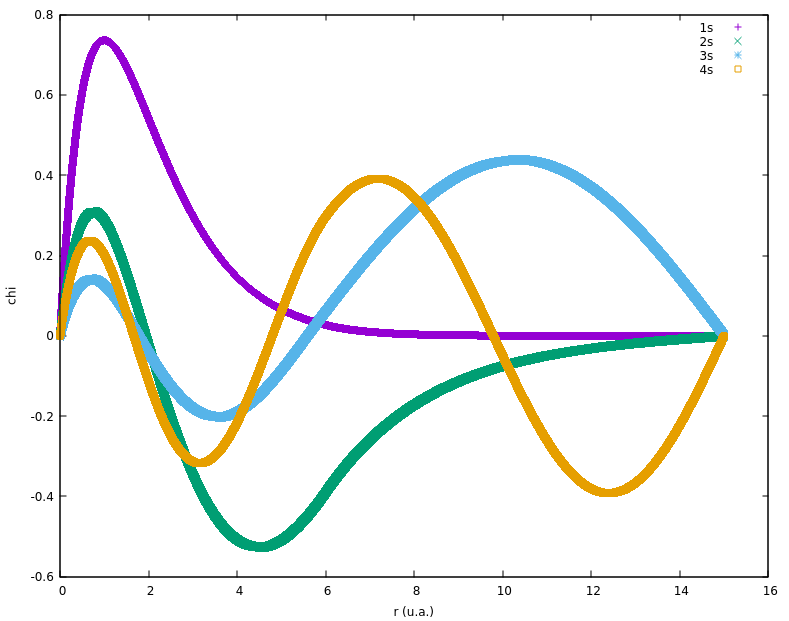
\includegraphics[scale=0.7]{4ss.png}
\caption{$\chi$ de los primeros 4 orbitales s del H, con $r_c=6.0$ y un limite superior de 15.\label{4ss}}
\end{figure}

\begin{figure}[h]
\centering
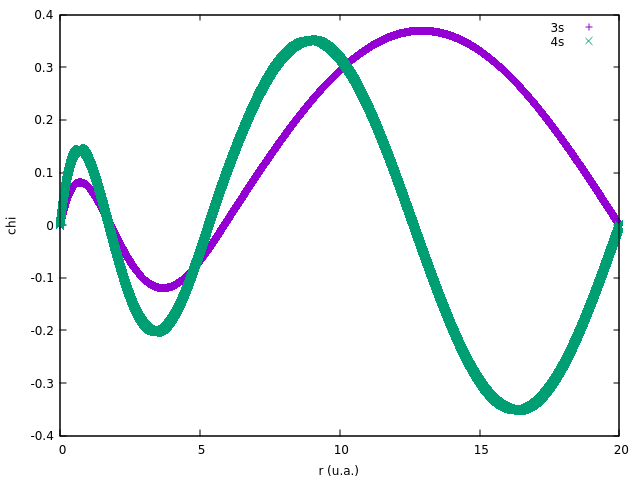
\includegraphics[scale=0.8]{3s4s.png}
\caption{$\chi$ de los orbitales 3s y 4s del H, con $r_c=6.0$ y un limite superior de 20.\label{3s4s}}
\end{figure}

En la Figura \ref{3pp} se muestran las $\chi$ obtenidas para los estados 2p, 3p y 4p del H; al igual que en el caso de los orbitales s, observamos que el 3p y 4p llegan de forma brusca al cero, y que el primer máximo del 4p es mayor al del 3p. Esta diferencia es mayor a la observada con el 3s y 4s, lo cual es esperable ya que los orbitales p están más distribuidos que los s y requerirán que se considere un infinito práctico mayor. En la Figura \ref{1s2p} se comparan las $\chi$ de los orbitales 1s y 2p, donde puede apreciarse que tienen una forma similar, pero con el máximo desplazado. Adicionalmente, en la Figura se muestran las $\chi$ obtenidas para los orbitales 3d y 4d utilizando 30000 puntos en la malla, dado que al usar el valor previamente usado el programa no arroja resultados. En este caso se observa el número adecuado de nodos y el máximo del 4d por debajo del máximo del 3d, pero se presenta una distorsión en la forma del 3d cerca del radio de corte.

\begin{figure}[h]
\centering
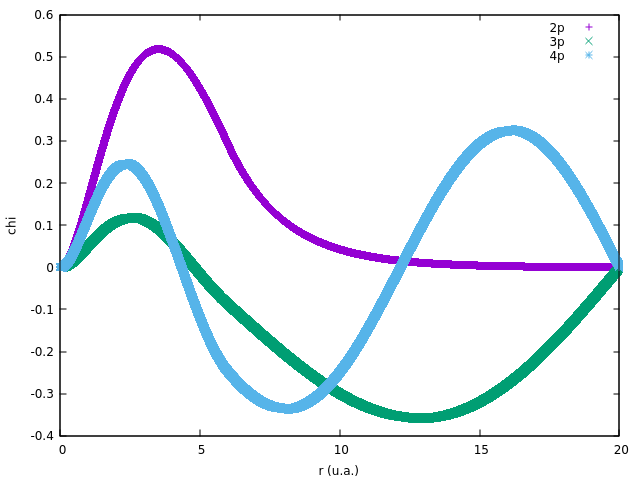
\includegraphics[scale=0.8]{3pp.png}
\caption{$\chi$ de los primeros 3 orbitales p del H, con $r_c=6.0$ y un limite superior de 20.\label{3pp}}
\end{figure}

\begin{figure}[h]
\centering
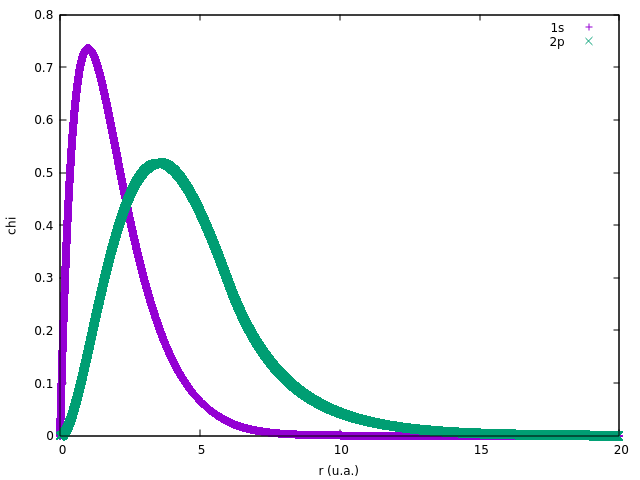
\includegraphics[scale=0.8]{1s2p.png}
\caption{$\chi$ de los orbitales 1s y 2p del H, con $r_c=6.0$ y un limite superior de 20.\label{1s2p}}
\end{figure}


\begin{figure}[h]
\centering
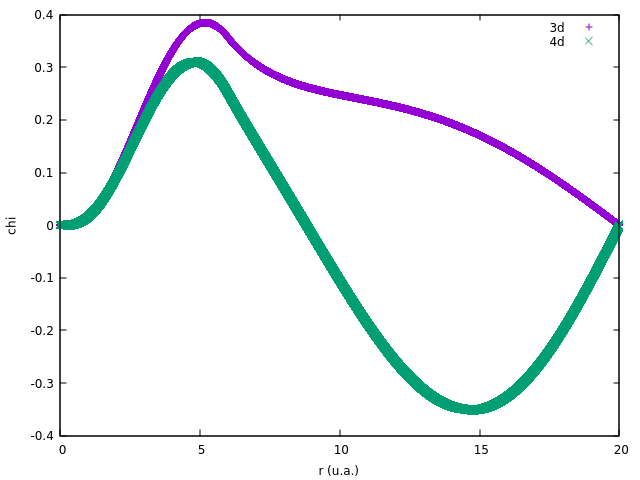
\includegraphics[scale=0.8]{2dd.png}
\caption{$\chi$ de los primeros 2 orbitales d del H, con $r_c=6.0$ y un limite superior de 20.\label{1s2p}}
\end{figure}


En el caso del átomo de H libre se espera que las energías de los orbitales 2s y 2p sean iguales, dado que esta solo depende de n (ecuación \ref{hene}). Esto no es cierto cuando el átomo de H se encuentra confinado: en la Tabla \ref{tab2} se comparan los valores de energía de orbitales con el mismo valor de n, utilizando valores de radio de corte de 2.0, 6.0 y 12.0. En ambas comparaciones es notorio como, conforme el radio de corte es menor, la energía asociada al orbital aumenta hasta ser incluso mayor a cero. Además, las energías entre los orbitales con un mismo valor de n dejan de ser iguales, pero comienzan a ser más semejantes conforme aumentamos el radio de corte y nos acercamos al caso de la partícula libre. En la Figura \ref{2src} se muestra como cambia el comportamiento de $\chi$ para el orbital 2s conforme aumentamos el radio de corte. 

\begin{table}[h]
\centering
\begin{tabular}{|c || c|c||c|c||}
\hline
$r_c$ & $E_{2s}$& $E_{2p}$&$E_{3s}$&$E_{3p}$\\
\hline
2.0   & 0.014925& 0.024954 & 0.059390 & 0.072073\\
6.0   & -0.084165& -0.102830 & 0.024715 & 0.028305\\
12.0   & -0.124201& -0.124625 & -0.033457 & -0.025762\\
\hline
\end{tabular}
\caption{Valores obtenidos de $E$ en Hartrees para orbitales con n igual. Para $r_c$ igual a 2.0 y 6.0 los resultados se obtuvieron con 666667 puntos en la malla, mientras que para $r_c=12.0$ se usaron 500000 puntos. En ambos casos se uso un infinito práctico de 20. \label{tab2}}
\end{table}

\begin{figure}[h]
\centering
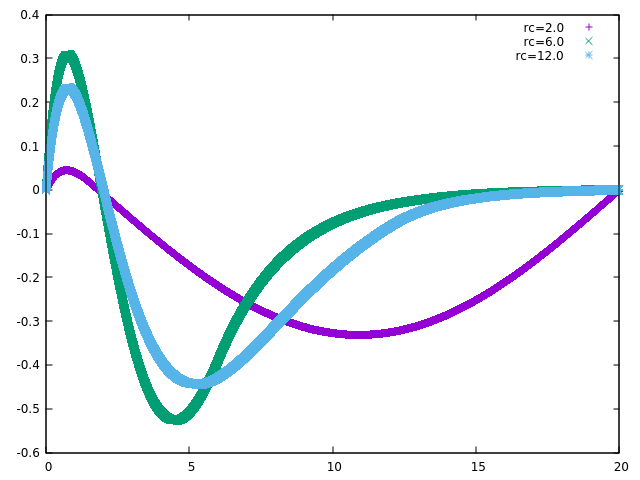
\includegraphics[scale=0.8]{2src.png}
\caption{$\chi$ del orbital 2s del H, con diferentes valores de $r_c$ como se indica en la gráfica.\label{2src}}
\end{figure}

Finalmente, de las distintas $\chi$ obtenidas calculamos la $R(r)$ asociada, dividiendo los resultados entre $r$. En las Figuras \ref{1sR}, \ref{2sR} y \ref{3sR} se muestran las funciones radiales de orbitales con el mismo valor de n, usando un radio de corte de 6.0. Claramente el comportamiento de dichas funciones concuerda con el que esta reportado en la literatura.

\begin{figure}[h]
\centering
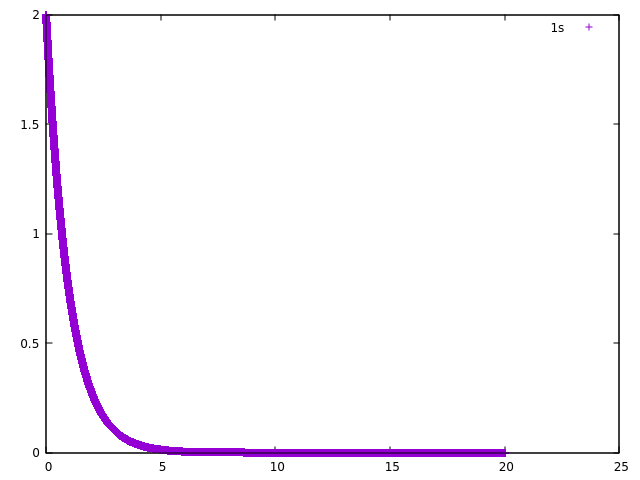
\includegraphics[scale=0.8]{1sR.png}
\caption{$R(r)$ del orbital 1s del H, con $r_c=6.0$.\label{1sR}}
\end{figure}

\begin{figure}[h]
\centering
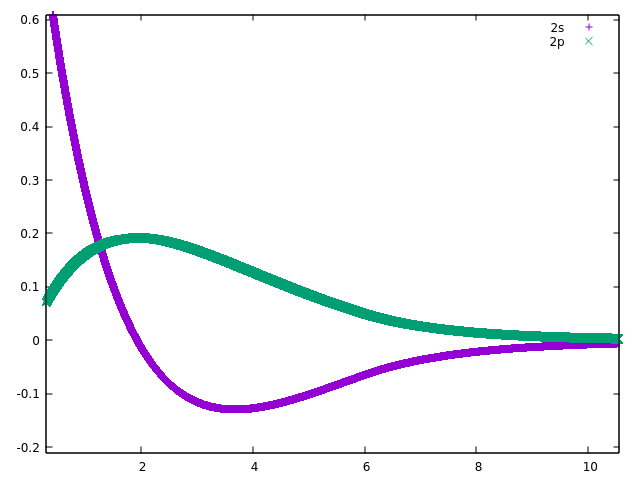
\includegraphics[scale=0.8]{2sR.png}
\caption{$R(r)$ del orbital 2s y 2p del H, con $r_c=6.0$.\label{2sR}}
\end{figure}

\begin{figure}[h]
\centering
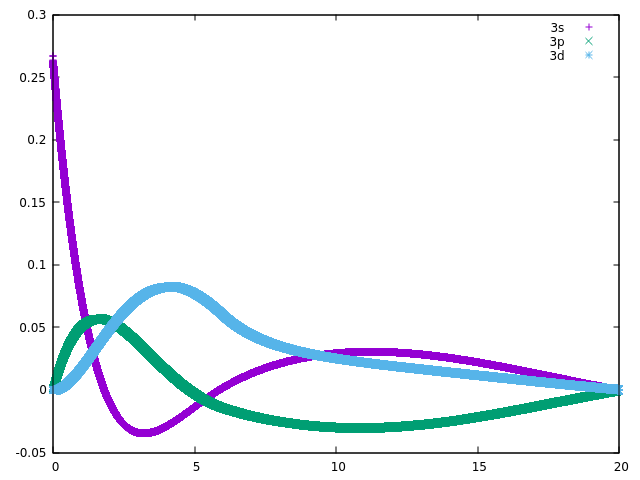
\includegraphics[scale=0.8]{3sR.png}
\caption{$R(r)$ del orbital 3s, 3p y 3d del H, con $r_c=6.0$.\label{3sR}}
\end{figure}

\subsection*{Conclusiones}

Mediante el método de Numerov es posible obtener buenos resultados para la parte radial de la función de onda del átomo de hidrógeno, pero resulta muy importante tener cuidado en la elección de los parámetros involucrados en el cálculo, ya que el método depende bastante de una buena elección de $h$, de la precisión de las variables utilizadas y la elección de un infinito práctico adecuado para el orbital que se desee reproducir.

Con el programa obtenido, fue posible obtener resultados interesantes para radios de corte del potencial variados para diferentes orbitales, con lo cual simulamos algunas situaciones de confinamiento del átomo de H. De estos resultados, es importante rescatar la importancia del uso de valores adecuados del radio de corte según deseemos observar situaciones de gran o nulo confinamiento para un tipo de orbital dado, ya que los resultados pueden corresponder para orbitales de bajos $n$ y $l$ al caso libre, mientras que para valores distintos de estos números cuánticos los efectos de confinamiento ya resultan importantes.

\end{document}